\documentclass{article}

\usepackage{amsmath,amsthm}
\usepackage{url}
\usepackage{graphicx}

\newcommand{\newword}[1]{{\bf #1}}
\newtheorem{problem}{Problem}
\newtheorem{theorem}{Theorem}
\newcommand{\NP}{\ensuremath{\mathcal{NP}}}

\title{Using Cell Phone Keyboards is (\NP) Hard}
\author{P. Boothe}

\begin{document}
\maketitle

\begin{abstract}
Sending text messages on cell phones which only contain the keys 0-9 and \# and
* can be a painful experience.  We consider the problem of designing an optimal
mapping of numbers to sets of letters to act as an alternative to the standard
$\{2\to\{abc\}, 3\to\{def\}\ldots\}$.  Our overall goal is to minimize the
number of buttons that must be pressed to enter an aferage message in English.
We prove that the problem in almost all of its variations is \NP hard, but
describe several mappings which improve the standard one.  With luck, one of
these new mappings will achieve success similar to that of the Dvorak layout
for computer keyboards.
\end{abstract}

Typing on a keyboard which has fewer keys than there are letters in the
alphabet can be a painful task.  There are a plethora of input schemes which
attempt to make this task easier, but the one thing they all have in common is
that all of these input methods use the standard mapping of numeric keys to
alphabetic numbers of 
$\{2\to\{abc\},
         3\to\{def\}, 4\to\{ghi\}, 5\to\{jkl\}, 6\to\{mno\}, 7\to\{pqrs\},
         8\to\{tuv\}, 9\to\{wxyz\}\}$.
However, if we don't mind breaking some ``legacy'' applications of the phone
system such as ``1-800-FLOWERS'', then we might try rearranging the numbers on
the keys to make messages easier to type.  Most variants of this problem turn
out to be NP-hard, unfortunately.

Before we get any farther, let us sketch the basic problem that we will keep
revising and revisiting throughout this paper.
\begin{problem}[{\sc MinimumKeystrokes}]~\\
{\sc Instance}: A set of letters corresponding to an alphabet $A$ $(|A| =
n)$, a number of keys $k$, an input method $IN$, and a set of
tuples of words and frequencies $W$.  The frequencies in $W$ are integers,
and the words are made up of solely of elements of $A$.  We will
treat $IN$ as a function which, given a partition of $A$ and a word
$w$, returns how many keystrokes are required to type $w$.~\\
        ~\\
{\sc Question}: What is the best partition of $A$ into $k$ sets, such that the
total number of keystrokes to type every word in $W$ its associated frequency
times is minimized?  Equivalently, what is the partition of $P$ of $A$ ($|P| = k$) that
will minimize
$$\sum_{(w,f)\in W} f*IN(w,P)$$
\label{probtemplate}
\end{problem}


Over the course of this paper we consider three different real-world
schemes for $IN$ (basic typing, T9, and predictive T9), and for each
variant that is proven \NP-hard, we consider the restriction on $P$ that
requires that we keep the alphabet in alphabetical order.  In all cases
where it is computationally feasible we provide results for the case of
the English language, on 8-key keyboards, using the British National
Corpus\cite{bnc} (BNC).  One feature of note is that no matter what scheme we
use, the problem is trivial if the number of keys is not smaller than the
number of letters in the alphabet ($k \ge |A|$).  Using tiny keyboards is only
(computationally) difficult when the keyboards don't have enough keys.

\section{Setting a Baseline with the Easiest Problem}

The baseline we compare against is the most painful method of text entry.  I
imagine that no ``digital native'' actually uses this input method, and that it
is available on all phones solely that their parents might use it.  In this
method, to type an `a', the user of the cellphone types the `2' key; to type a
`b' they type `22', to type `c' they type `222', to type a `d' they type `3',
to type an `e' they type `33', and so on.  To type a word with multiple
letters that use the same key, such as `accept', the user must pause
between keystrokes.  Thus, the full key entry sequence for `accept', using
`.' to indicate a pause, is `2.22.223378'.

\begin{figure}
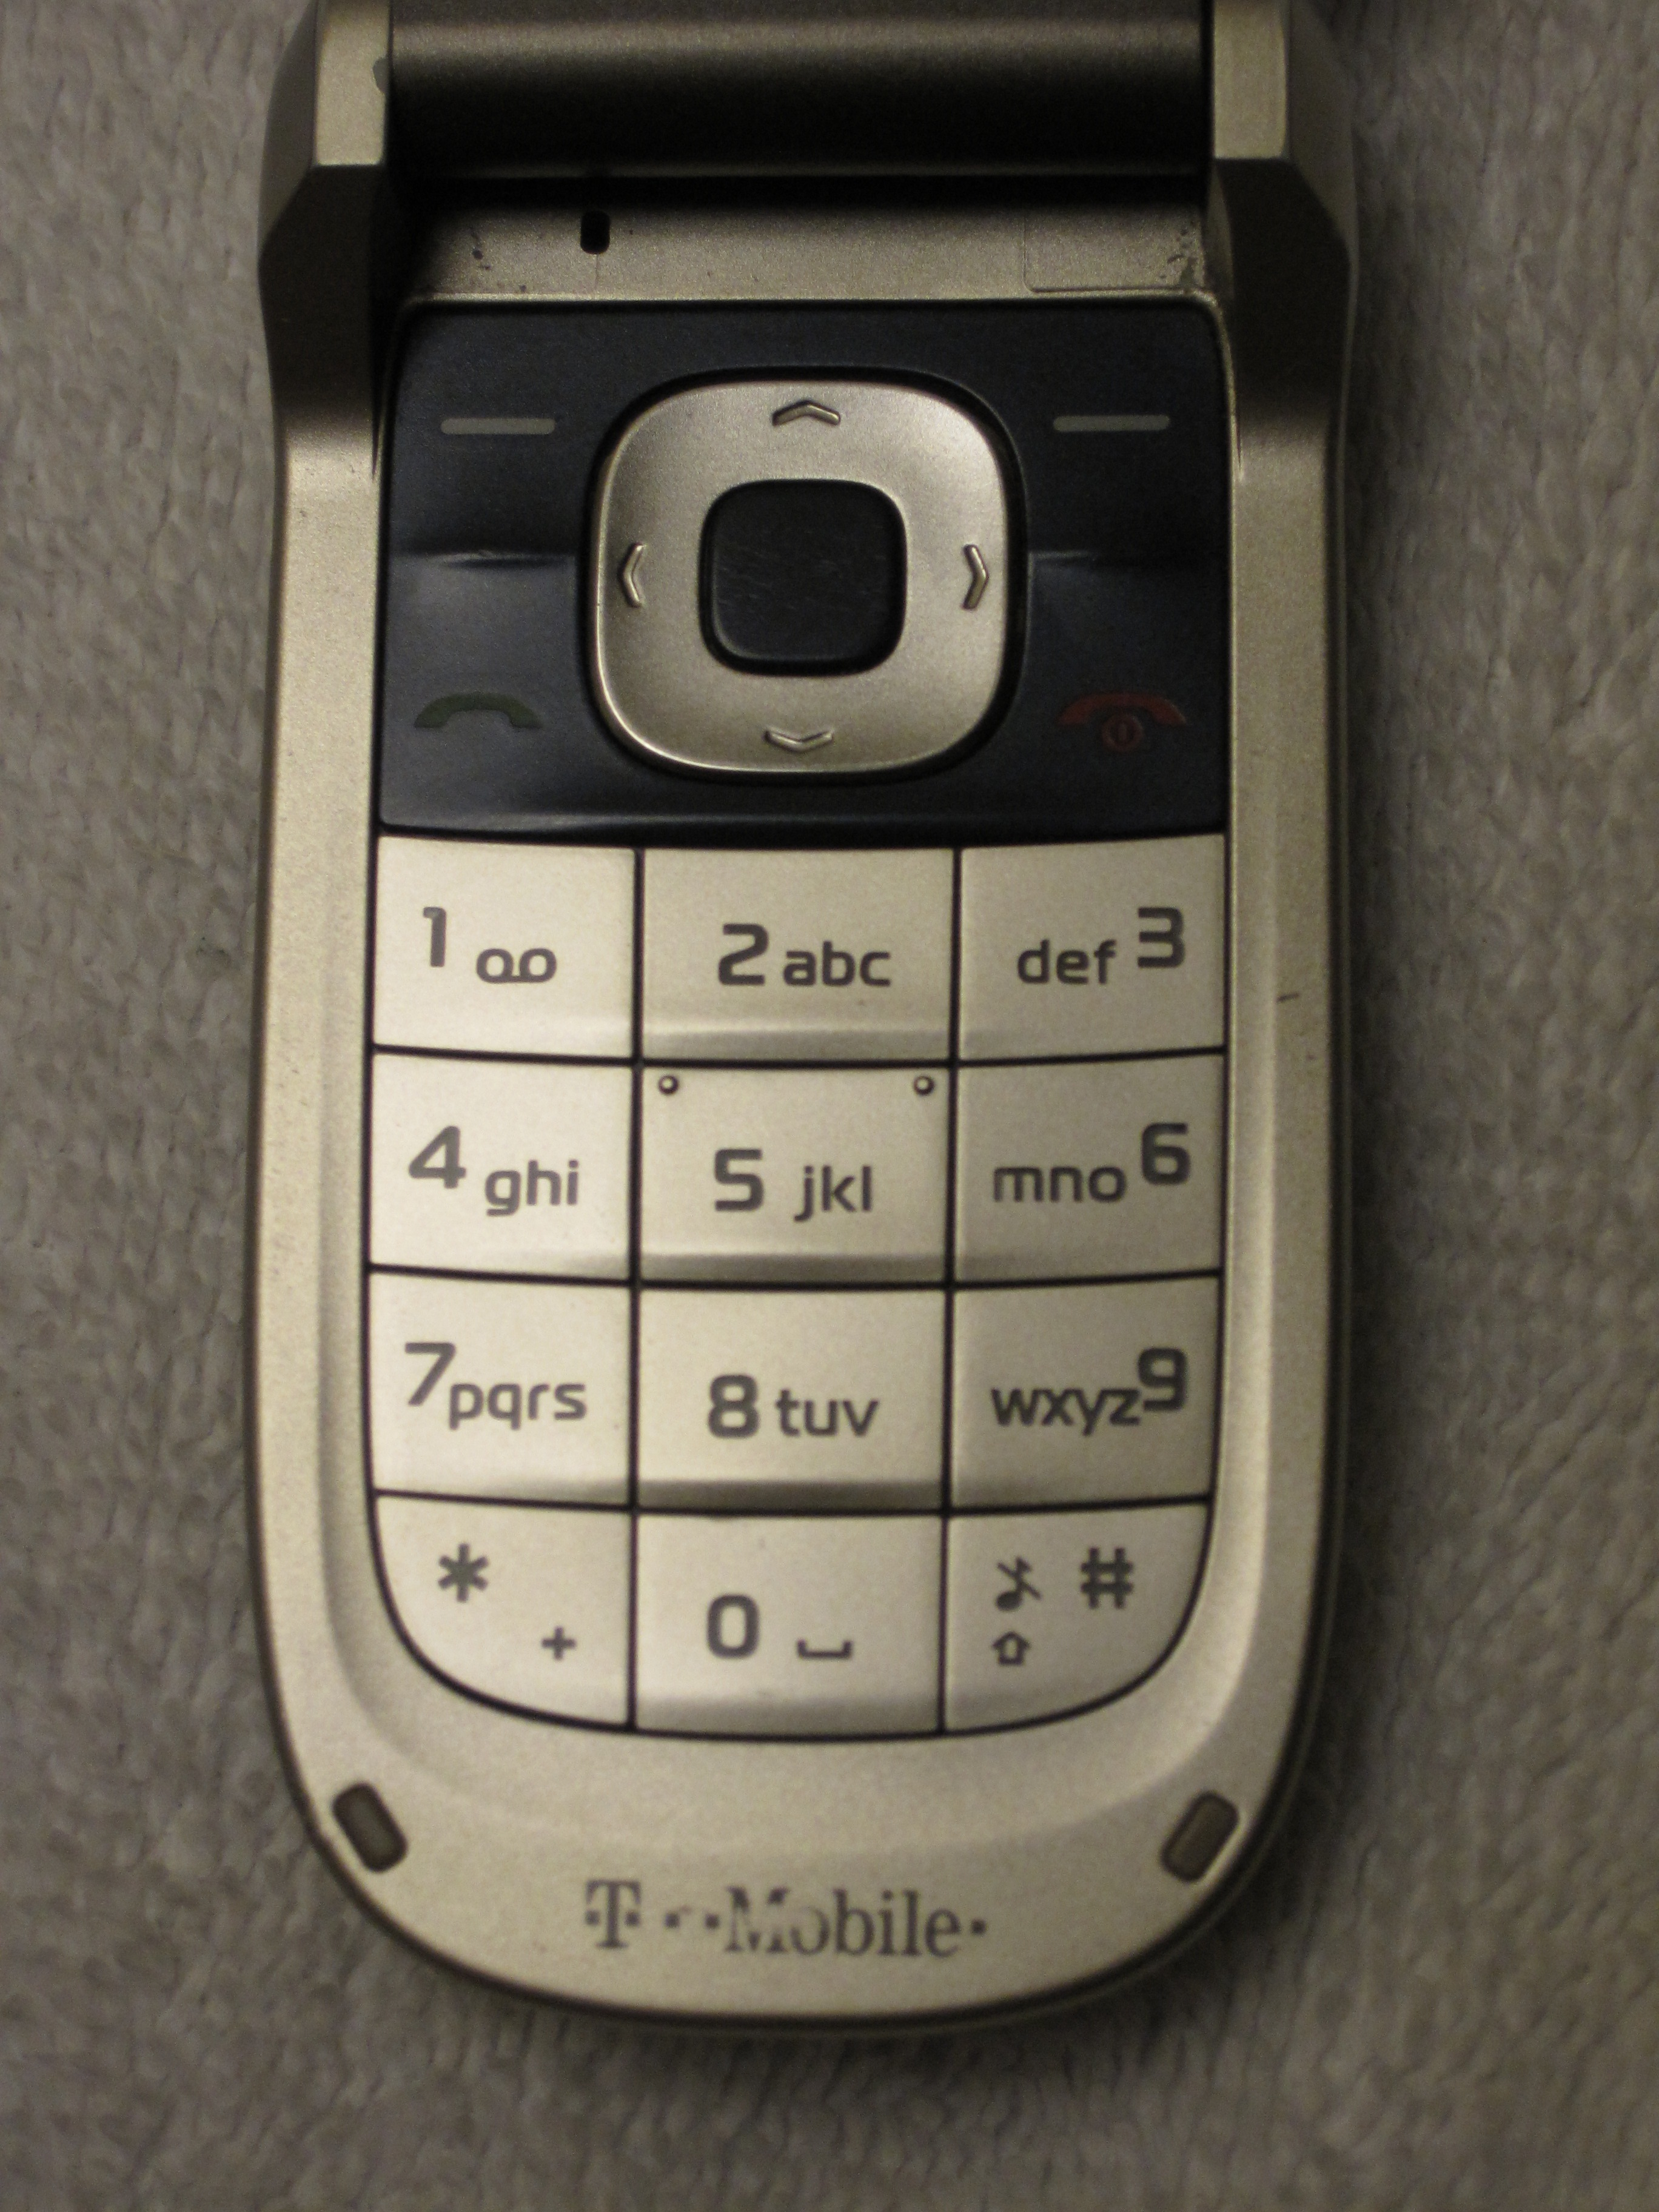
\includegraphics[width=2in]{phonekeys.jpg}
\caption{A cell phone keyboard}
\label{keypic}
\end{figure}

Initially, we will completely neglect the pauses and concern ourselves solely
with the number of keystrokes required.  This implies that `a' will always
require one button press, `b' will always require two, and so on.  Thus, to get
a baseline of how many keystrokes are required to enter the entirety of our
corpus of words $W$, we count the total number of occurences of each letter,
and multiply that number of occurrences by the number of button pushes
required by that letter.  Running this on the British National Corpus
using the standard cell phone keyboard layout, we find that entering the
entirety of the 100,106,029 word occurrences in the corpus would require
948,049,046 button presses.  

If we examine a cell phone keyboard (Figure~\ref{keypic}) then we can see that
there are some terrible choices being made.  The frequently-occurring letters
'r' and 's' require more keystrokes than 'q'!  Surely, a better designed
keyboard can do better than this.  If we just reversed the order of the letters
on the 7 key, from `pqrs' to `srqp', the number of button presses required
would drop to 865,118,331 --- a savings of more than $8.7\%$!  If we assume
that every button press takes an equal amount of time, then this corresponds
the users spending $8.7\%$ less time entering their text messages.  In an
effort to find out how low this can go, we define the problem {\sc
BasicCellPhoneTyping} based on the template problem on
page~\pageref{probtemplate}.

\begin{problem}[{\sc BasicCellPhoneTyping}]~\\
{\sc Instance}: A set of letters corresponding to an alphabet $A$ $(|A| =
n)$, a number of keys $k$, and a set of
tuples of words and frequencies $W$.  The frequencies in $W$ are integers,
and the words are made up of solely of elements of $A$. \\
        ~\\
{\sc Question}: What is the best partition of $A$ into $k$ sequences, such that the
total number of button presses to type every word in $W$ its associated frequency
times is minimized?  The number of button presses is equal to the order of the
letter in the sequence assigned to a given key.  For example, in the key
$2\to\{abc\}$, $a$ requires one keystroke and $c$ requires 3.
\label{probtemplate}
\end{problem}

Unlike almost every other problem dealing with key assignment, we can construct
an efficient algorithm for this problem.  We can construct a provable optimal
greedy algorithm which works in time $O(|W| + |A| \log |A|)$.  Our algorithm is
detailed in Figure~\ref{greedyalg}, and involves creating a histogram of the
letters, and then assigning letters to keys round-robin style in the order from
most-popular to least-popular.  To prove optimality, we invoke an exchange argument.

\begin{theorem}
The greedy algorithm finds an optimal solution to {\sc BasicCellPhoneTyping}.
\label{basicthm}
\end{theorem}
\begin{proof}
We will assume, for simplicity of proof, that all letters occur a different number of times in the corpus.  
We begin by comparing two assignments of letters to keys by, for each assignment,
constructing a sequence of sets, or spectrum, $S$.  The set $S_1$ (layer 1) is the set of all
letters which require a single button press (that is, they are the first
letter in their sequence on their assigned key), $S_2$ (layer 2) is the set of
all letters which require two button presses, and so on.  If two assignments
have the same sequence of sets, then one assignment may be transformed into
the other assignment simply by swapping letter between keys without
increasing or decreasing the total number of button pushes required to enter
the corpus of words.  If two sequences have equal spectra, then we say their corresponding assignments are isomorphic.

Now assume for the sake of contradiction that we have assignment $D$, with spectrum $T$, that is not isomorphic to the greedy solution $G$ with spectrum $S$.
Note that in spectrum resulting from the greedy algorithm, all letters at layer
$i$ occur strictly more frequently than the letters at layer $j$, $j > i$.
Also, in $S$, for all layers $i$ except for the last layer, $|S_i| = k$.
Because $T$ and $S$ are not isomorphic, in $T$ there must be at least one layer $i$ such that $T_i \neq S_i$.  Let $T_i$ be the first layer for which that is true.

There are two cases for layer $T_i$.  In the first case, $T_i < k$, and we may
remove any element from a later layer and create a strictly better layout.  In
the second case, there is some letter $a$ such that $a \in T_i$ and $a \not\in
S_i$.  We choose the least-frequent such $a$.  Because the greedy layout
algorithm creates layers in order of frequency, we know that the frequency of
$a$ is less than that of some letter $b$ in layer $T_j$, $j>i$.  Therefore, by
creating a new layout with $a$ and $b$ swapped between $T_i$ and $T_j$, we have
strictly decreased the number of button presses.  Therefore, in both cases,
$T$ was not an optimal layout, and we have reached our contradiction.
\end{proof}

For the BNC, the optimal layout has the spectrum 
$$[\{etaoinsr\}, \{hldcumfp\}, \{gwybvkxj\}, \{qz\}]$$
and will require 638,276,114 button presses to
entire the entire corpus instead of our original requirements of
948,049,046.  This represents a savings of $32.67\%$ over our original
layout, but only for the case of users who type using the most basic of
input methods.  Unfortunately, this is the group of users who are likely
the least adaptable to change, as almost all ``digital natives'' use one of
the predictive methods to input text messages\footnote{I have no statistics
on this except for an informal survey of one of my classes.  In that
class, every student who used SMS either had a cellphone with a 26+
key alphabetic keyboard or used a predictive method.}.  If we would
like to place the least burden on these users whilst still
decreasing the number of button presses, we now consider schemes
where the only alteration of the keyboard is the rearrangement of
the sequence of letters for a given key.

By an argument symmetric to the proof of Theorem~\ref{basicthm}, we
find that the optimal layout in this new scheme is to place the letters of a
given key in sorted order.  Thus, the keyboard layout changes to $2\to[acb],
3\to[edf], 4\to[ihg], 5\to[lkj], 6\to[onm], 7\to[srpq],
8\to[tuv], 9\to[wyxz]$ and requires 678,547,463 button presses to
enter the whole corpus.  This represents a $28.43\%$ savings, but has the
added benefit that it does not change which key is mapped to which set of
letters.  Furthermore, it also is \newword{legacy preserving}, as
creating a keyboard with this layout will not invalidate such advertising
gems as 1-800-FLOWERS or 1-800-MARINES.  Thus, we can speed up users by
$28.43\%$ (neglecting inter-letter pauses) and not undermine 50 years of
phone advertising.  This layout represents perhaps the most plausible
layout yet.


\bibliographystyle{abbrv}
\bibliography{bibliography}
\end{document}
